\documentclass[sigconf]{acmart}

\usepackage{graphicx} %LaTeX package to import graphics
\graphicspath{{images/}} %configuring the graphicx package

\fancyhf{} % Remove fancy page headers 
\fancyhead[C]{Technical Report} % TODO: replace 9999 with your paper number
\fancyfoot[C]{\thepage}

\setcopyright{none} % No copyright notice required for submissions
\acmConference[Technical Report]
\acmYear{2023}

\settopmatter{printacmref=false, printccs=true, printfolios=true} % We want page numbers on submissions

%%\ccsPaper{9999} % TODO: replace with your paper number once obtained

\begin{document}
\title{Technical Report For Guardian} % TODO: replace with your title
\author{Noor Atieh, Ofek Sela, Gali Maman}
\begin{abstract}
In this project we wanted to help people save their privacy and secure their data especially their images, today exists AI model that can manipulate images from text description creating impressive results and anyone can use them with no effort such models are diffusion and styleGan. Here comes our role to make life harder for such models to edit or change images creating bad results and unrealistic images such protection methods are encoder attack and diffusion attack. To do so we designed a web application that allow users to upload images and get involve in protecting these images how they see fit while highly keeping their privacy during the usage of the application, our work relates and depends on pervious works. we also conduct user study to get a better understanding of the people thoughts about our work and how much we succeeded in making them feel more secure.
\end{abstract}

% TODO: replace this section with code generated by the tool at https://dl.acm.org/ccs.cfm
\begin{CCSXML}
<ccs2012>
<concept>
<concept_id>10002978.10003029.10011150</concept_id>
<concept_desc>Security and privacy~Privacy protections</concept_desc>
<concept_significance>300</concept_significance>
</concept>
</ccs2012>
\end{CCSXML}

\ccsdesc[300]{Security and privacy~Privacy protections}
% -- end of section to replace with generated code

\keywords{AI; Diffustion; styleGan; Diffustion attack; Encoder attack} % TODO: replace with your keywords

\maketitle

\section{Introduction}

In the recent years, the ability of editing face images, for example, using diffusion models and GAN models, has been significantly improved. As a result, people can no longer trust images they see on the internet, and people's personal images are at risk. Today even a teenager with basic knowledge in technology can edit images using AI to an extend better than an expert photo editor. This is not necessarily a bad thing however in the wrong hands and putting to bad use can actually create real harm to people and invading their privacy.  

We wish to create a simple but effective tool which would help people protect their images  at the same time Understand the risks and the damage that can be done if they neglected adding an extra layer of protection to their images. We did so by developing a web application in which users can try to use these AI models to manipulate images to be able to have a deeper understanding of the risks and the problem we are trying to solve we offer them two models, "diffusion and styleGan". we also give the users a mean to protect the images using two methods, "diffusion attack and encoder attack". In our web application we wanted to keep it basic focused and looking professional. 

The ability of running these AI manipulation models on their protected images and compare the results. Our goal is to make users feel same with their images posted on the internet.
here is an example of the capabilities of the AI today,just by inputting the image and text saying "man in the gym":

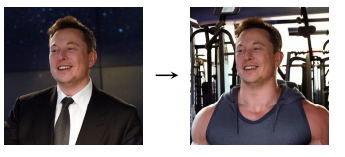
\includegraphics[width=0.4\textwidth]{exmple1}

We also seek to conduct a user study where we are asking people to go ahead and try our web application with all its features get a taste of it then having them in an interview still user study where we are going to ask them questions on a lot of aspects of their experience and usage and what changed from before trying our application to after. When enough people have participated and we have big enough data base we will analyses the results and people answers.      

Our web application is not finished and we are looking to expand on it in the future, according to users' feedback, in addition we still so many ideas that we weren't able to add for the shortage of time that we can add in the future.

We will expand on everything that was mentioned in the introduction in the next sections.     

\section{Related work}

Our project is based on three prior works. first one ~\cite{a}, in this paper explained how the diffusion model work and how to it take an image, mask and text prompt and return an edited image that is changed according to the text given to it. it also suggested two methods for immunizing images against diffusion model: diffusion attack and encoder attack, explaining how each one work and the advantages and disadvantages of each method . This work was a huge part of our project since other than the Information in the paper, the authors wrote a python code for diffusion model and the two methods of immunizing images here we took this code and customized to fit our need. 

the second one ~\cite{b}, this paper drove us deeper into the styleGan model and how it could manipulate images even though it is a face generation model and created to generate face images not edit exited images. StyleGan specially in face images only however since it works only on the images in its data base it doesn't do a good job editing images not in it's data base, when an image is uploaded it finds a face image in the data page that is close looking to the given image and manipulate the image in the data base. Yet we still wanted users to be able to run this model if they wanted so we added it to our project.

The third work ~\cite{c}, In order to make the stylegan model more userFriendly and similar to what we already have we decided edit via text we had to use styleClip which uses StyleGan but allow uploading images and edit these images via text and here we used their work sending all inputs to a secure server which run styleClip and return result.

\section{Methodology}

\subsection{Technical approach}

We choose to build our project using HTML (the bass for all web application), CSS(to desgin and create the outside look), Javascript(to handle all the iner workings of the web application), and Python creating a web application. we used Flask python library for the simplicity of it to combine python code and html code since all of our backend is written in python and frontend in html. We believe that a simple yet comfortable app, allow users to gain the most out from it even if they have little to no experience in the subject, and since the whole idea of our project is to allow users to protect their images and understand the risks we gave them the options to run all the models and the attacks on the same image and see the results side by side. As explained before we decided to give the user to AI models to manipulate the images diffusion and styleGan plus two methods to protect images being encoder attack and diffusion attack. for the styleGan we needed to make users edit the images with the simpliest way possible thus we used StlyeClip and even run the model on an external server making it lighter for our server to run it. we also focused on the feature of allowing users to customize their own target image for the immunization process since this will play a huge role on our user study. The web application contains 4 primary pages to keep it simple for user we went for more pages less option in each page design.

The first page only asks for user to upload an image then go to the second page where they can create the mask here users who wish to use diffusion model or any of the attacks have to paint the area to keep untouched to get better results, notice for those who wish only to use styleGan can skip this part as creating the mask won't affect the end results. From here we go to the most important page which is the settings page we decided that it would be best to just give the user to run whatever they want and not limit them to a number of options to run on the same image thus made it as check boxes for user to select from if a user wish to use immunization methods, he will have to choose a target image or a default one will be selected automatically. For styleGan he needs to feel a text describing what's in the image he wants to change, exp: user want to change the eye color of a woman. He should type: "woman with eyes". For all AI model if selected a prompt is needed describing what you wish to get. And at the end we move to results page here all the images that the user selected to create will be shown next to each other with a download button under each image that will allow him to download the image above it. One of the most important aspects is the performance for us since all the running of the AI models and methods to protect from them are very have on the server making it take such a long time to run, thus we suggest running the project using a very strong server otherwise it will be unusable. Another important aspect was the GUI (graphical user interface) we wanted the web application to look good and professional making it pleasant for the user to use our application. Lastly the features in the application plays a huge rule from the small ones to the necessary ones. Turning it from a basic primal application to a very neat professional one that will make the user experience much better.

Now we will present  an example of how our web applaction works in this example the user want to immunize his image with encoder attack and see the result when diffusion is applied to the image:

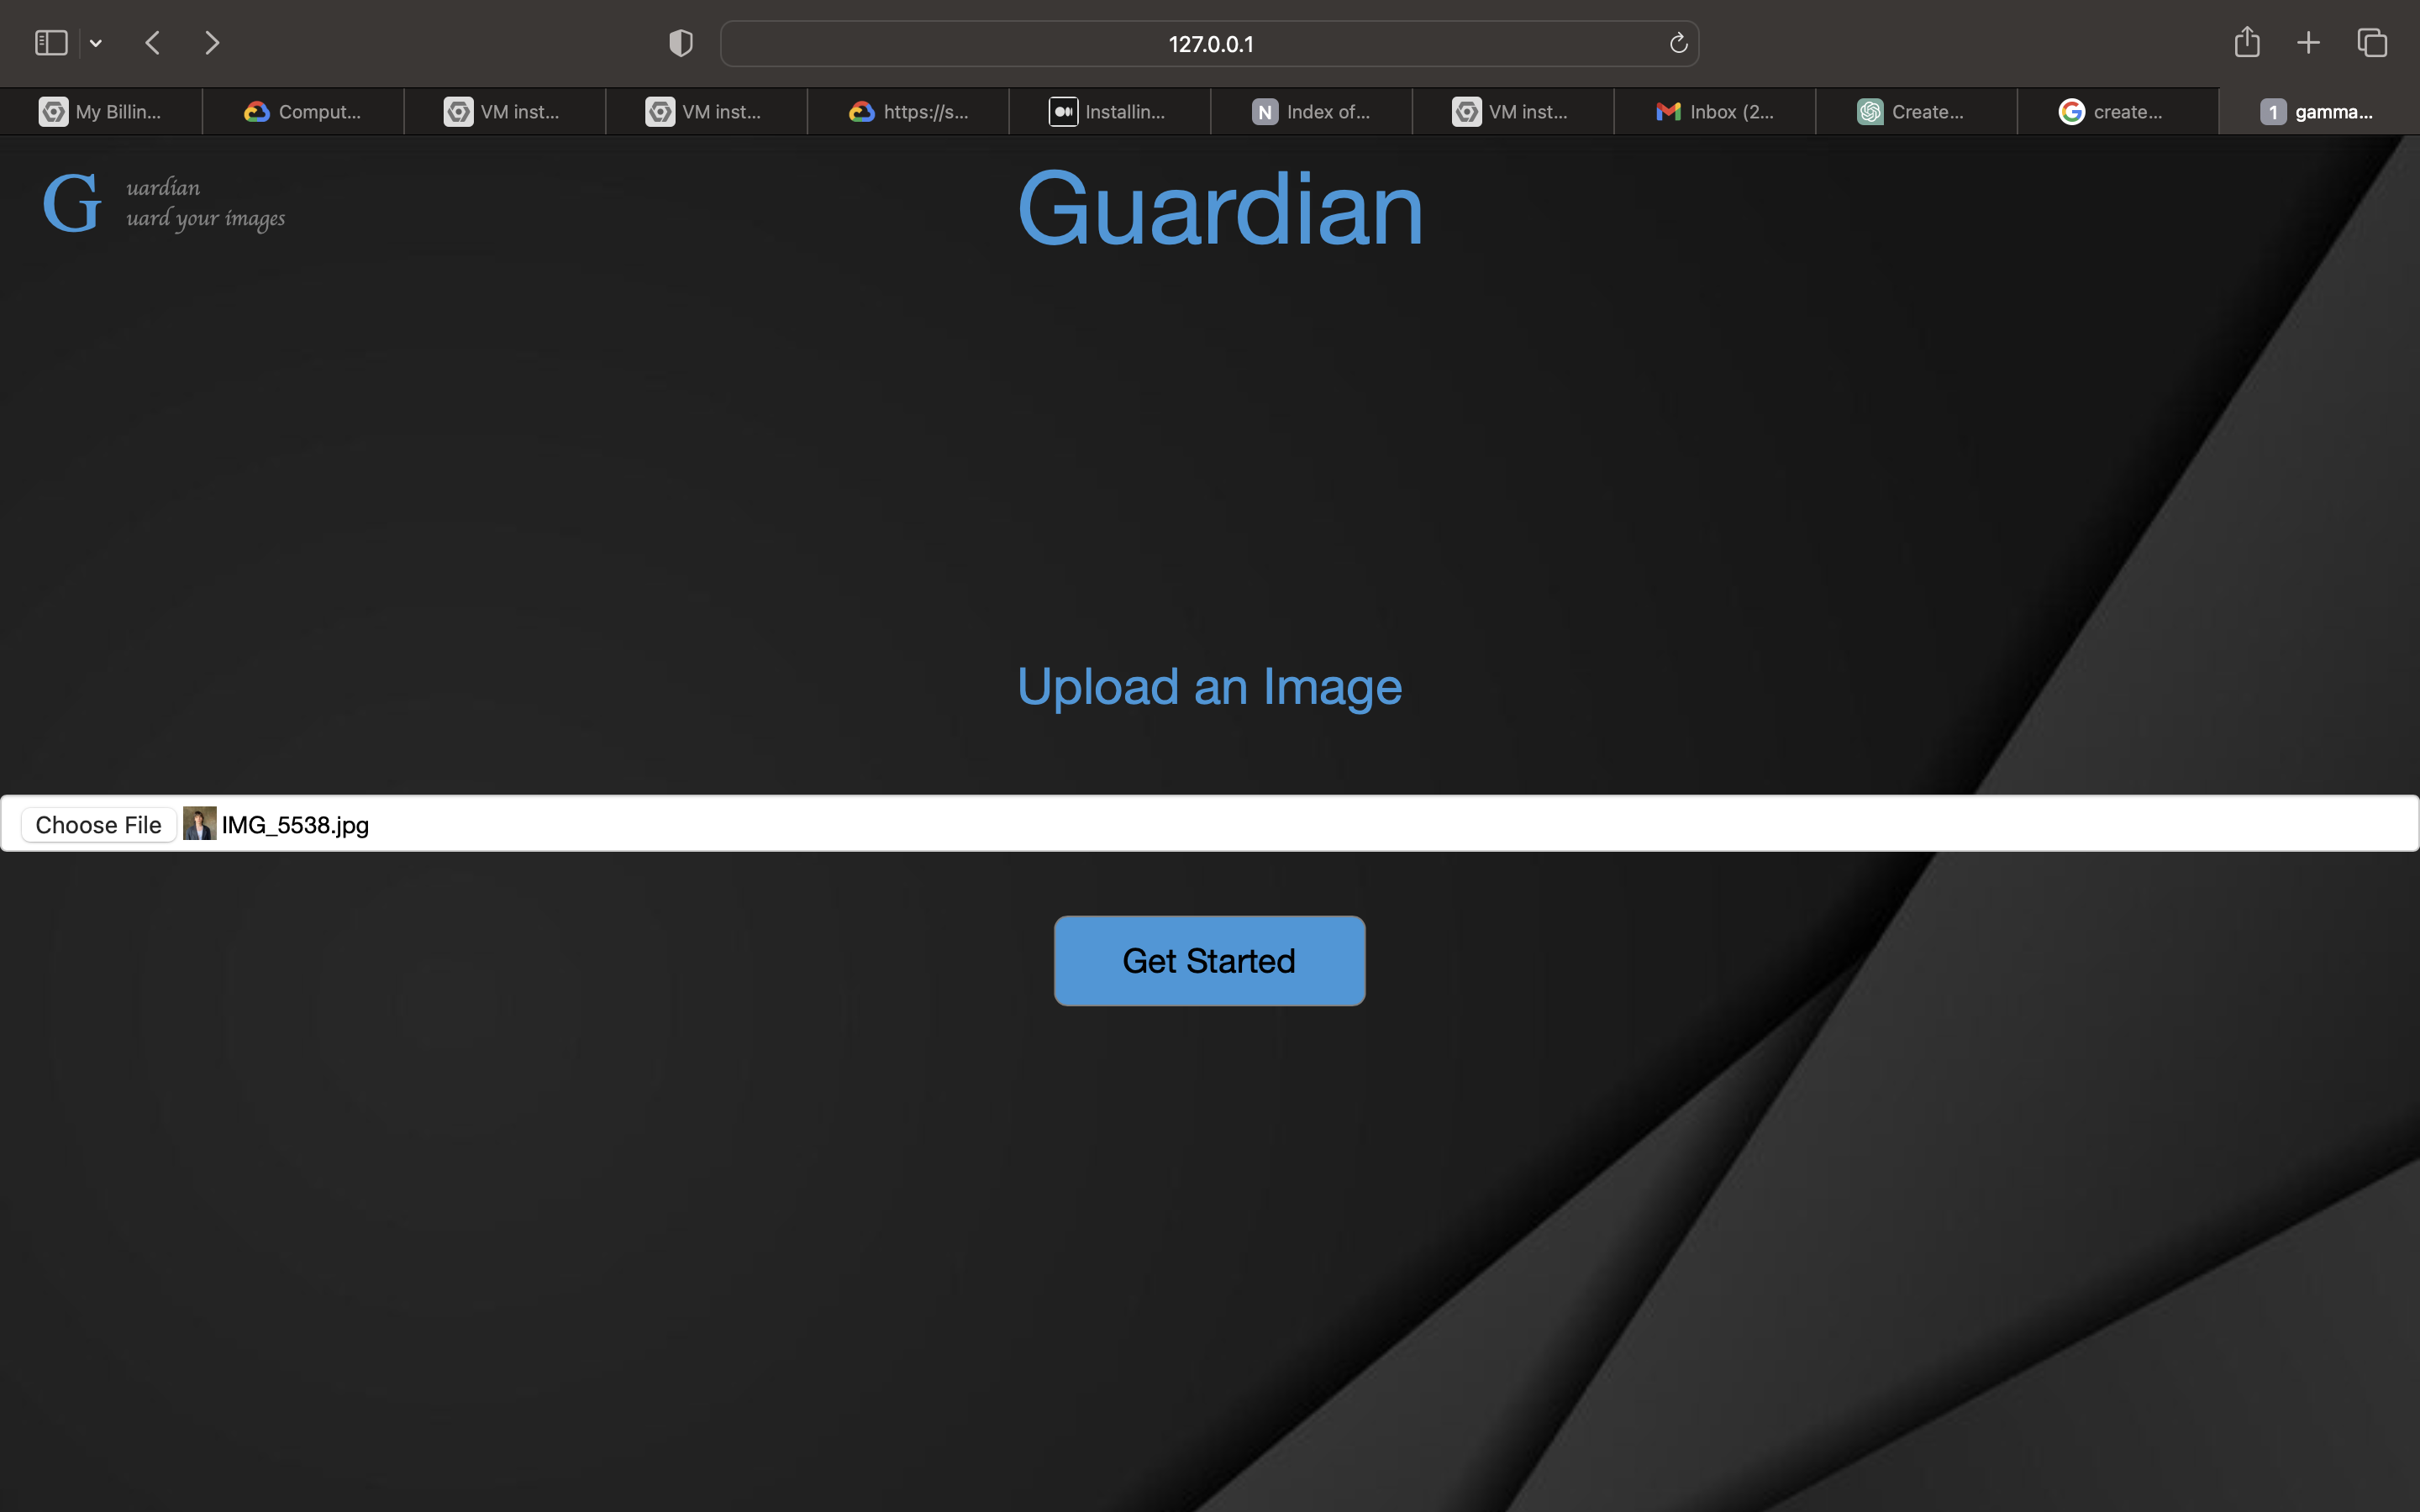
\includegraphics[width=0.4\textwidth]{1}

This is the home page of the website here users upload an image from their local machine.

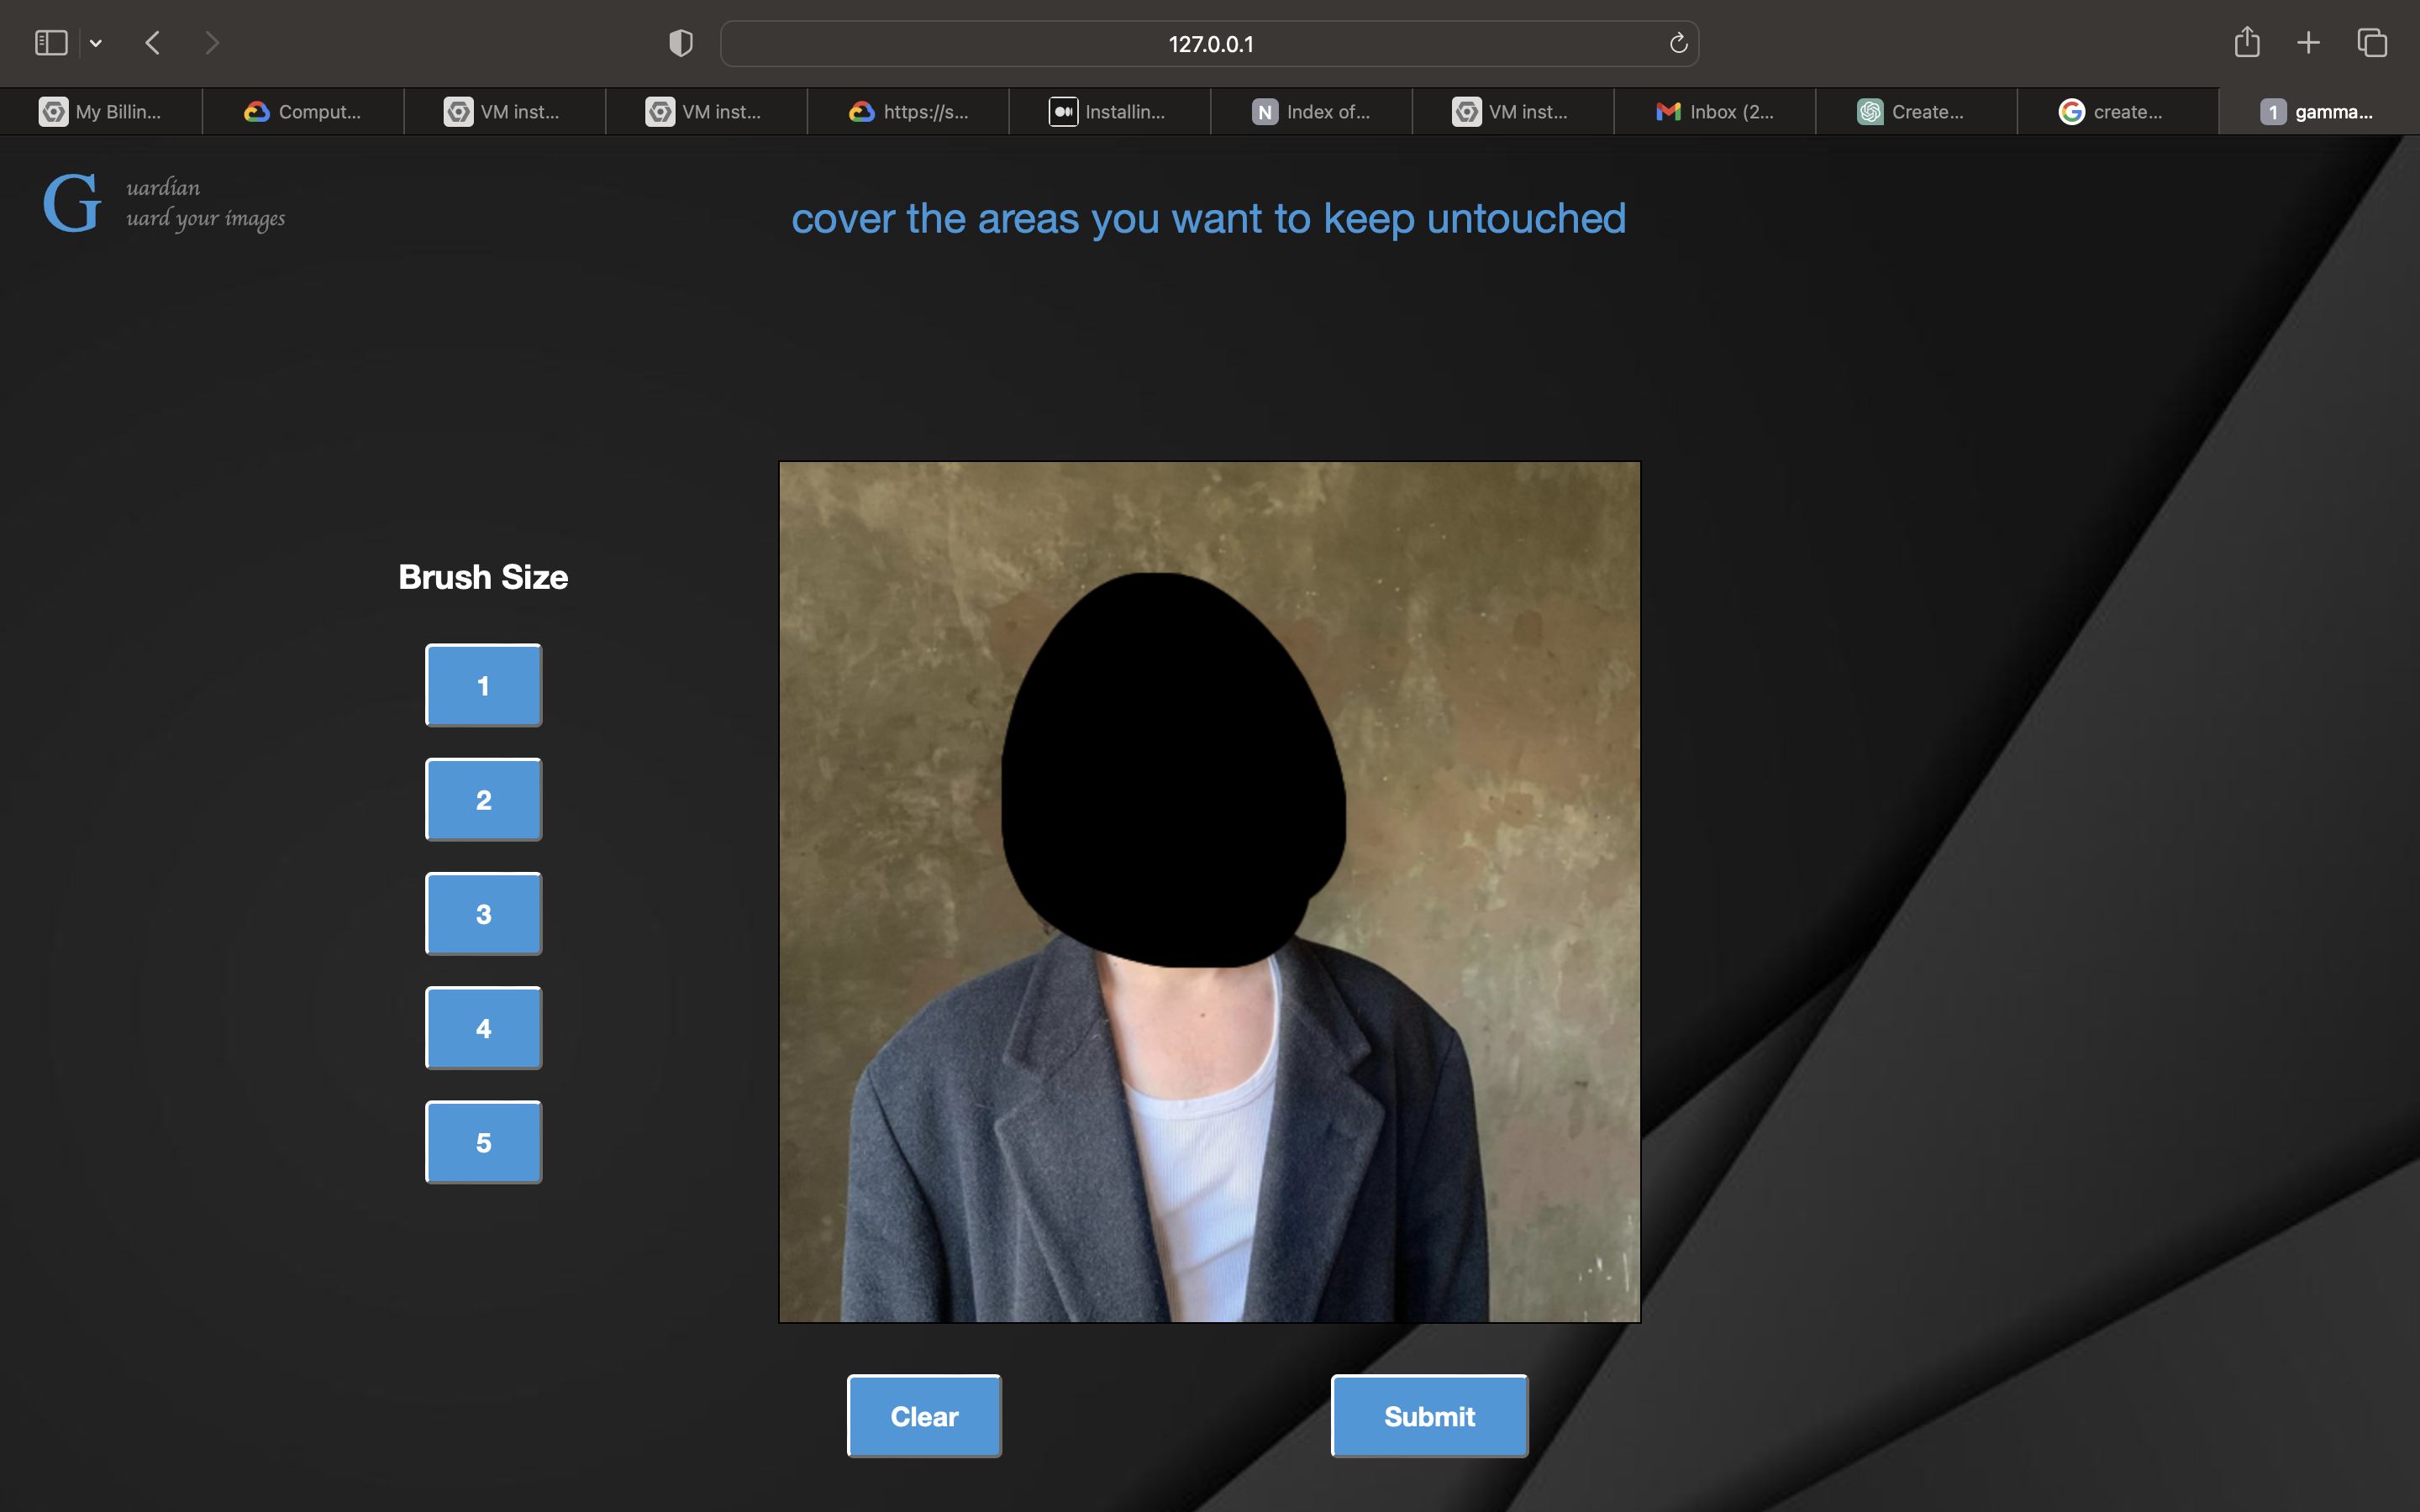
\includegraphics[width=0.4\textwidth]{3}

Here the user paint over the unchangable area since he wants to use diffusion.

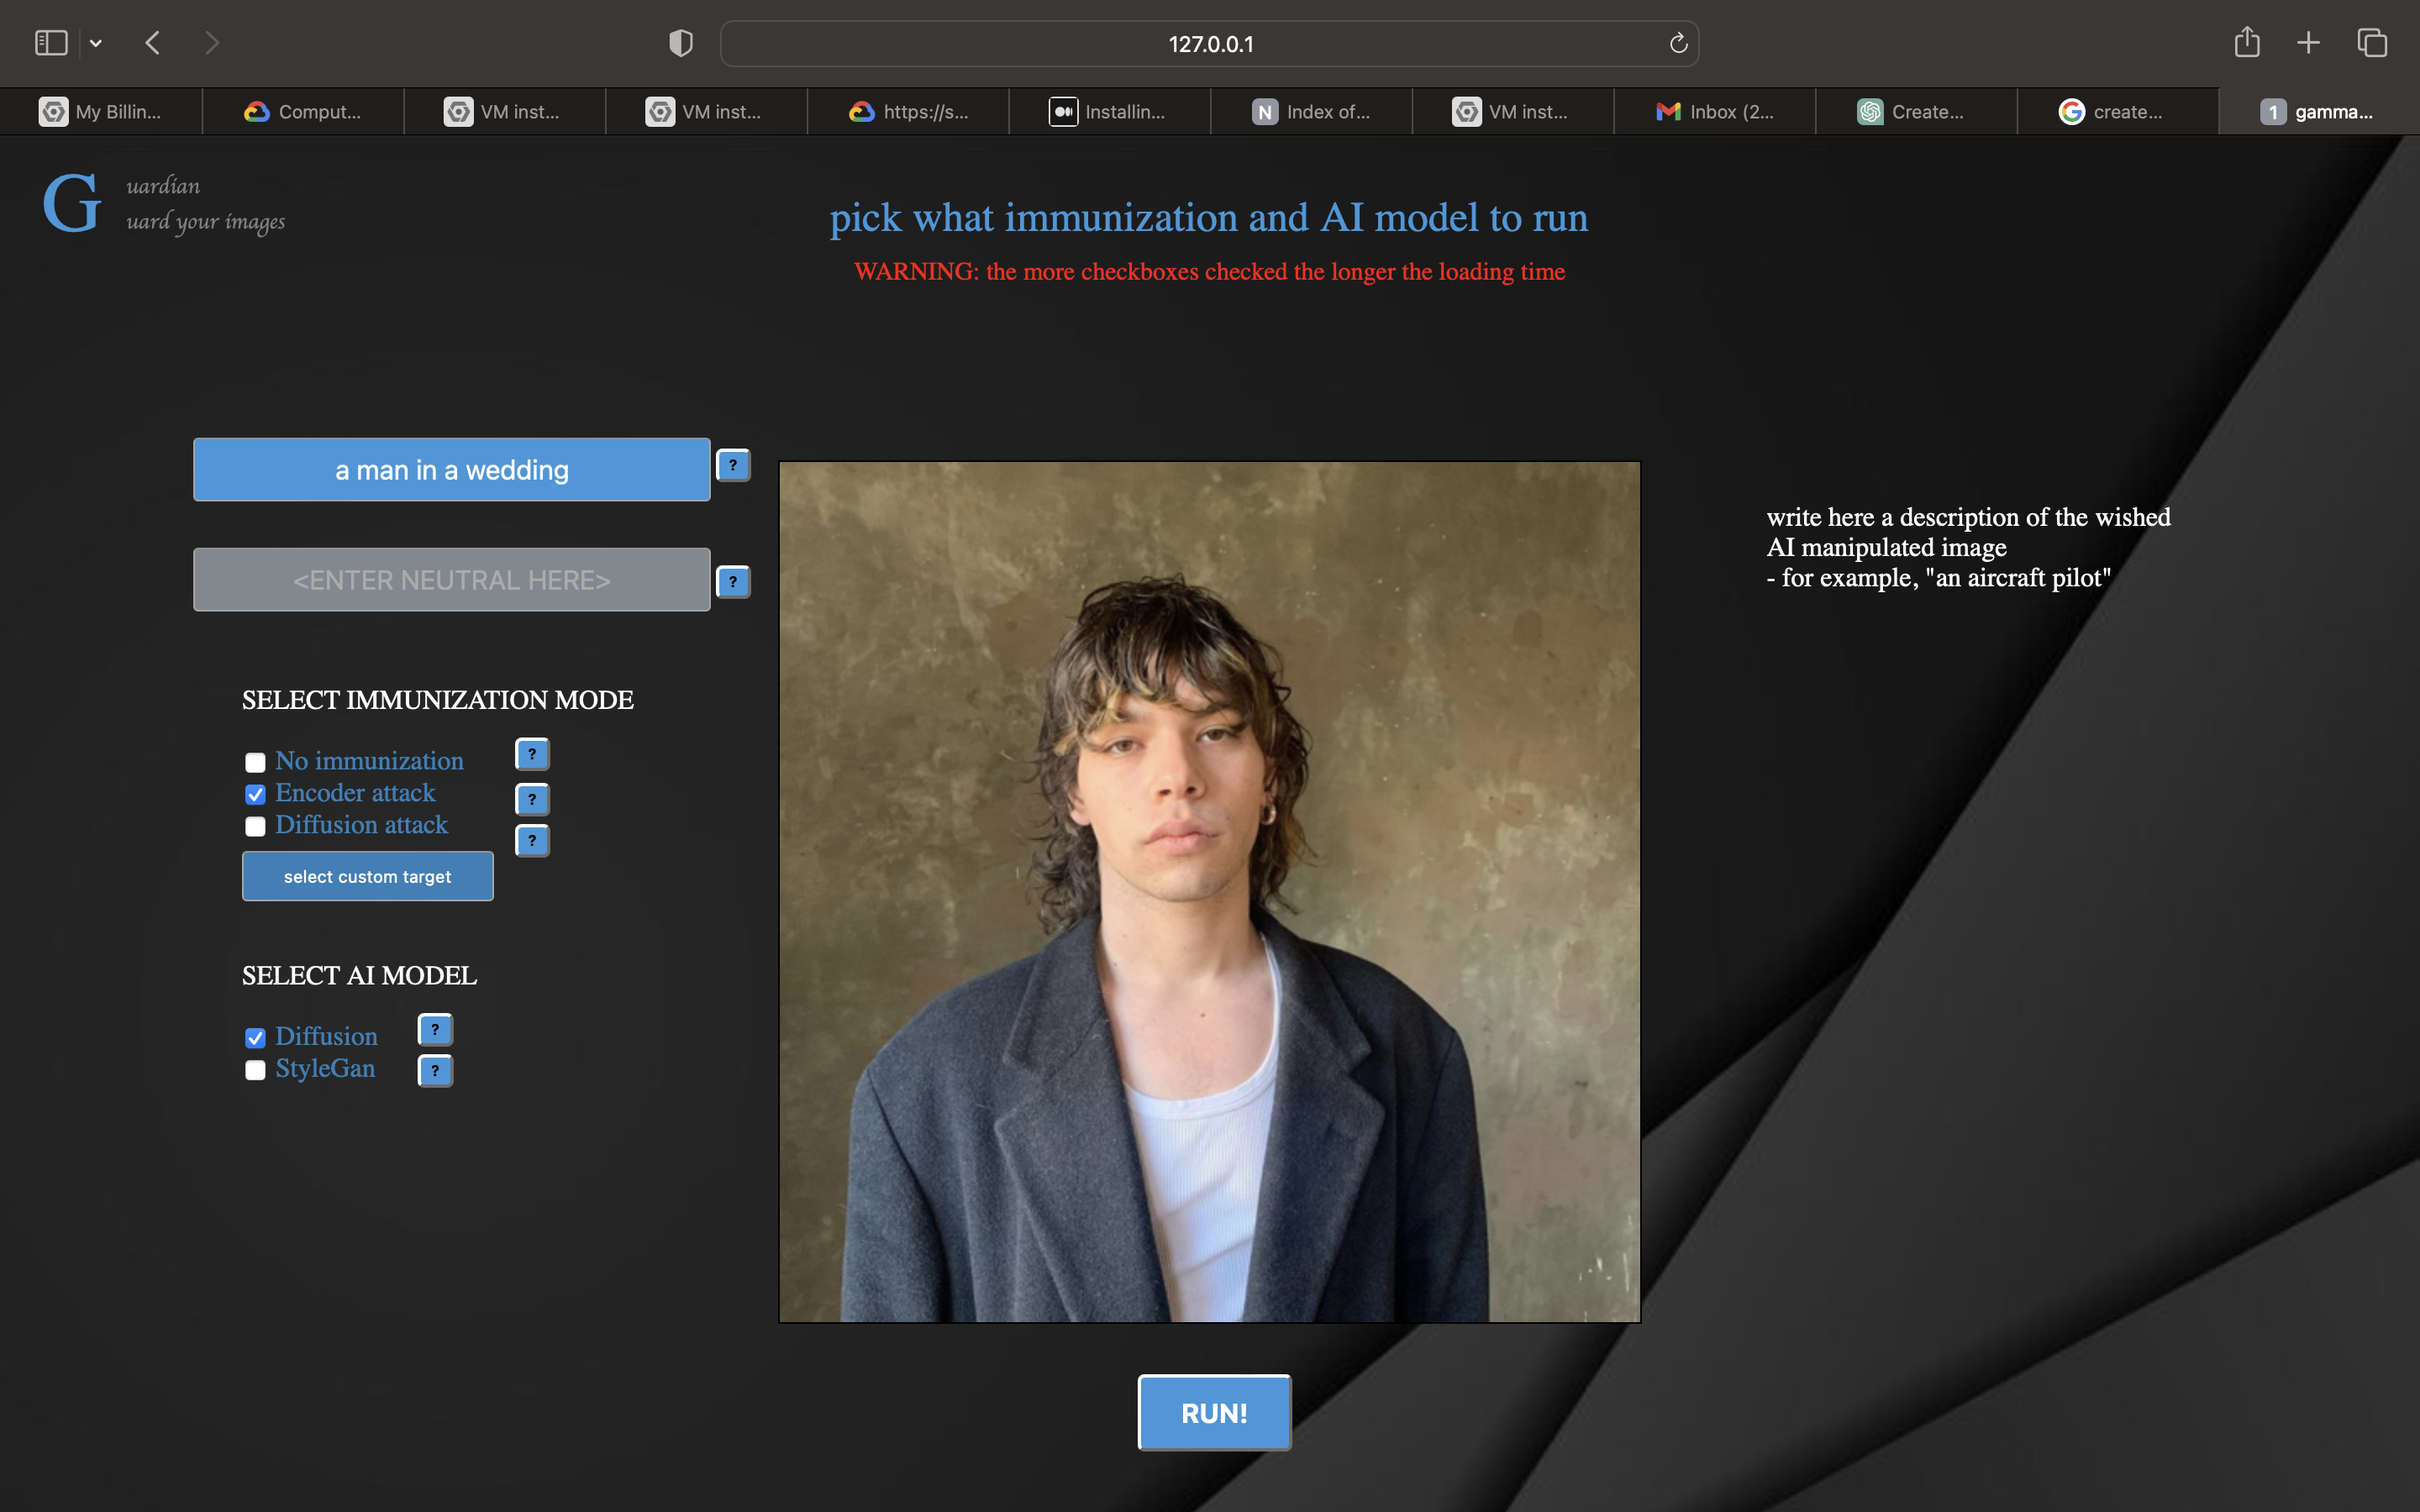
\includegraphics[width=0.4\textwidth]{4}

This is the settings page here users choose what they want to run.

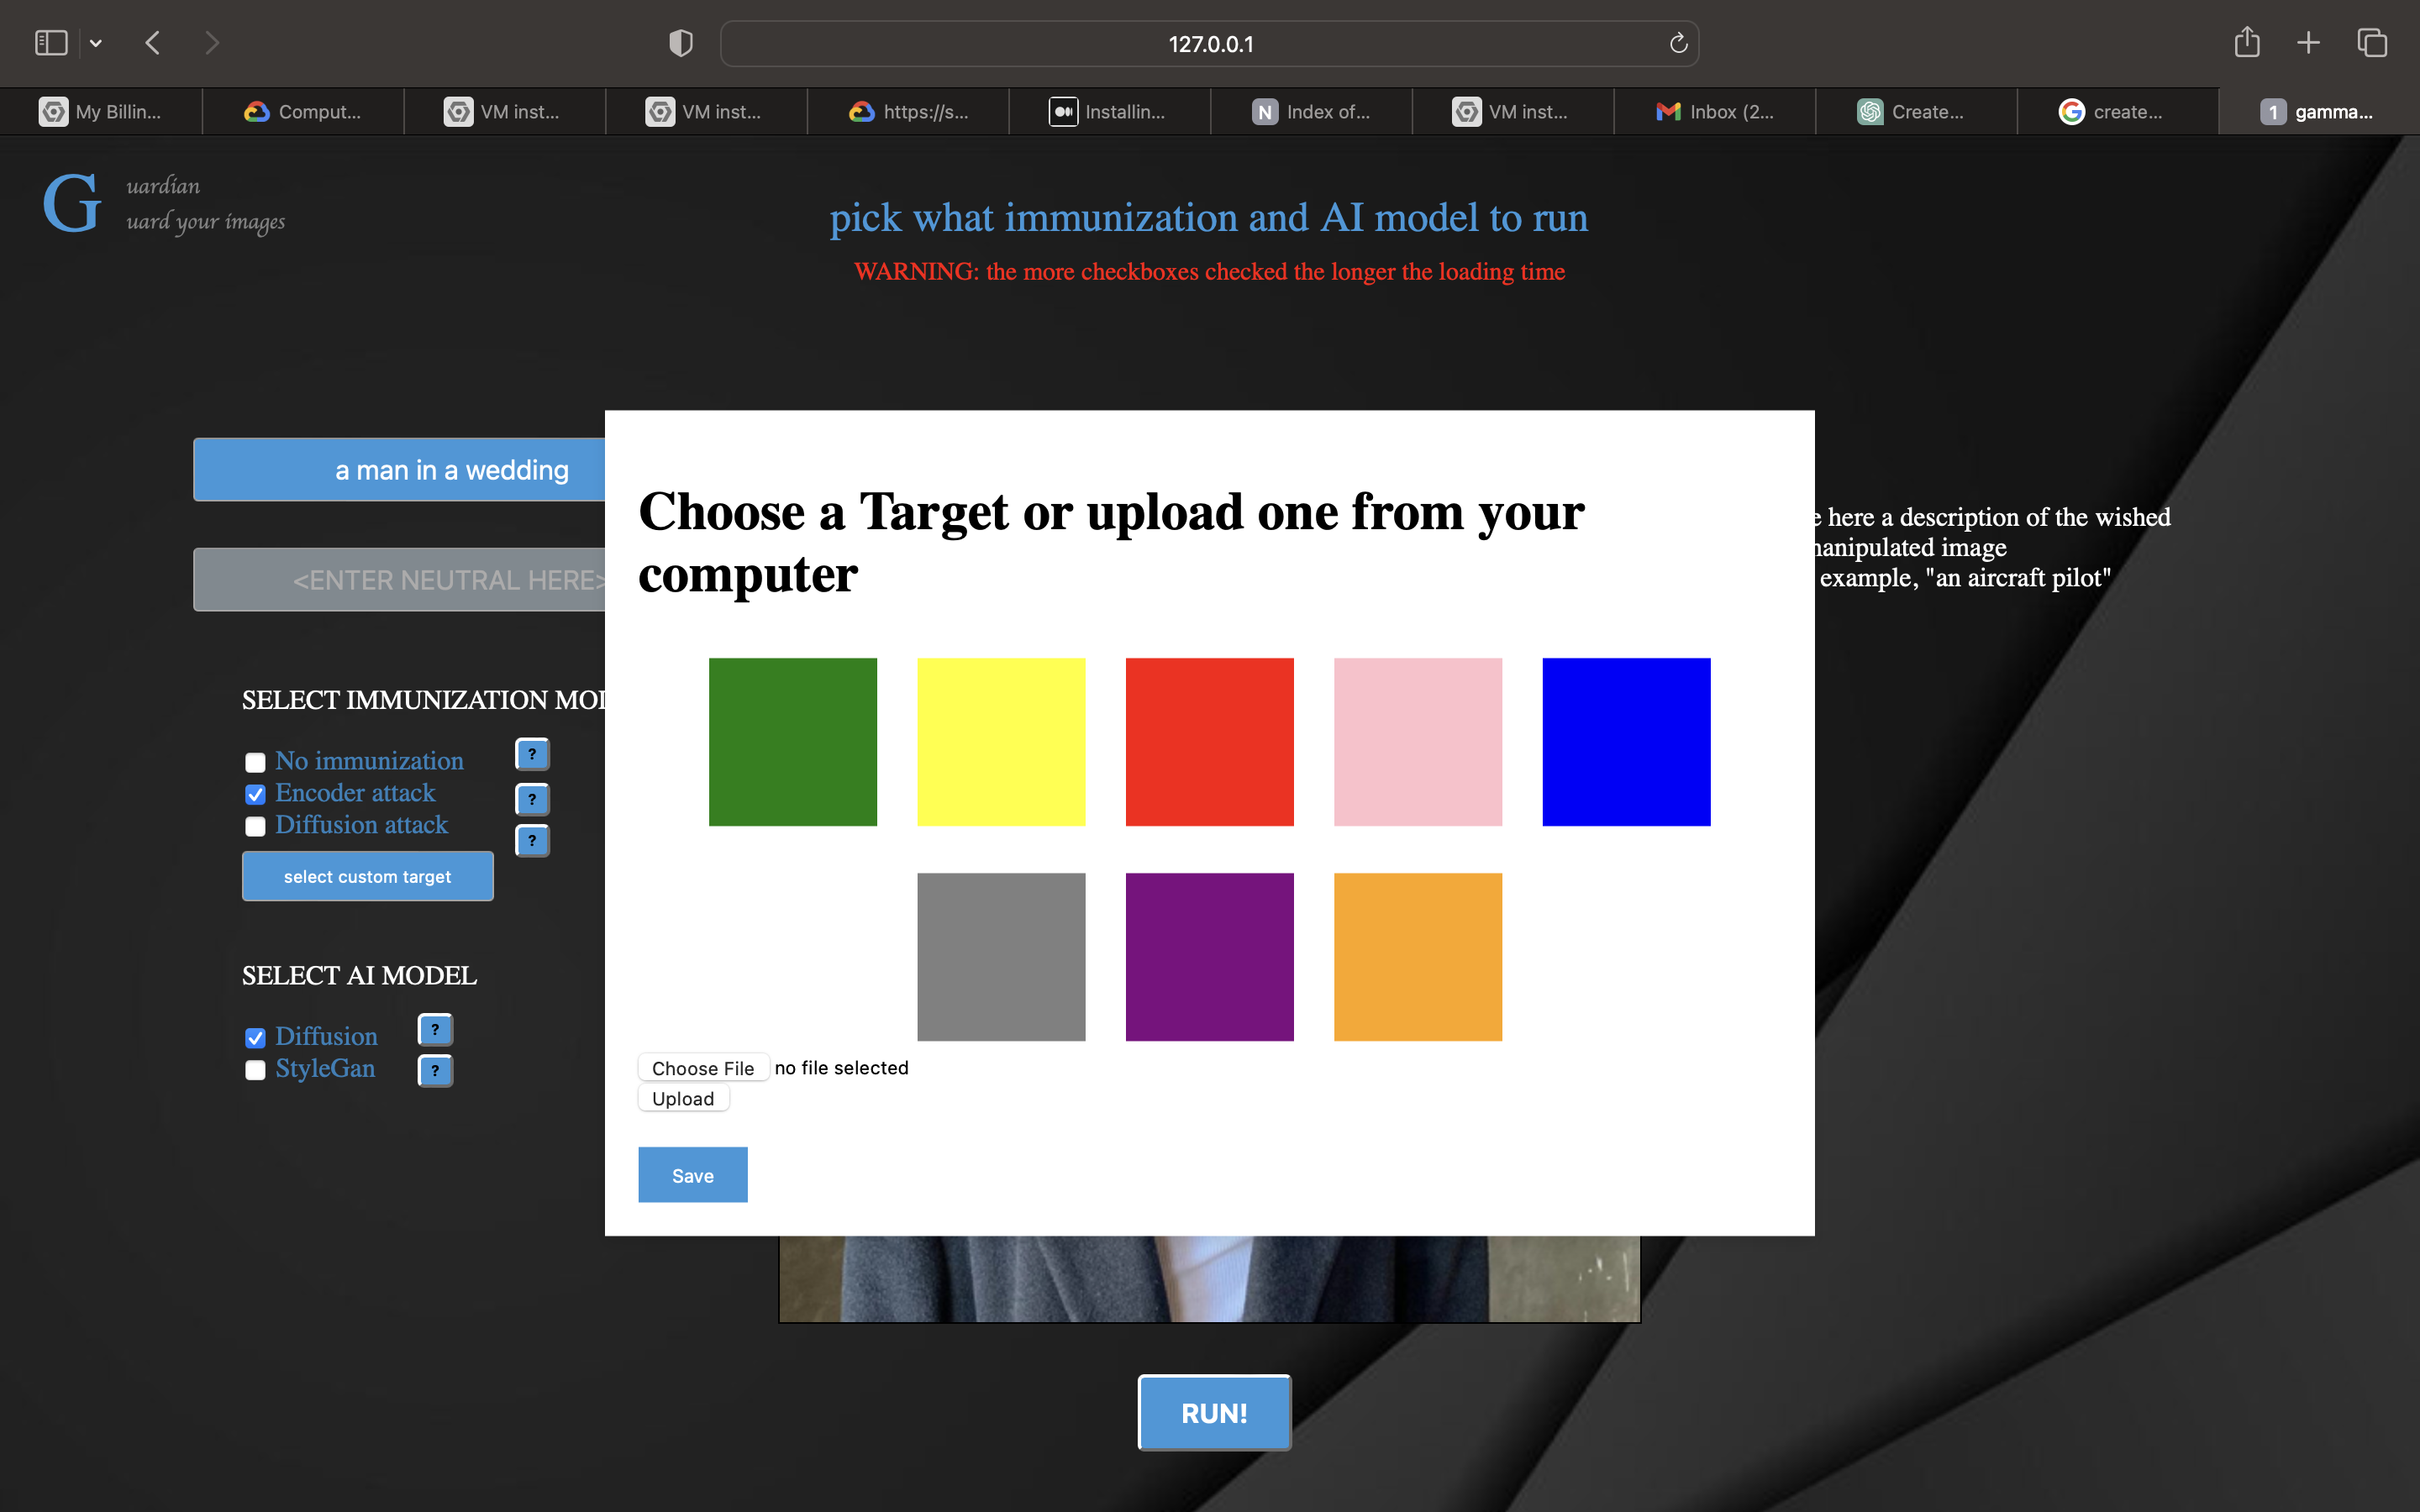
\includegraphics[width=0.4\textwidth]{2}

The user then choose a target image.

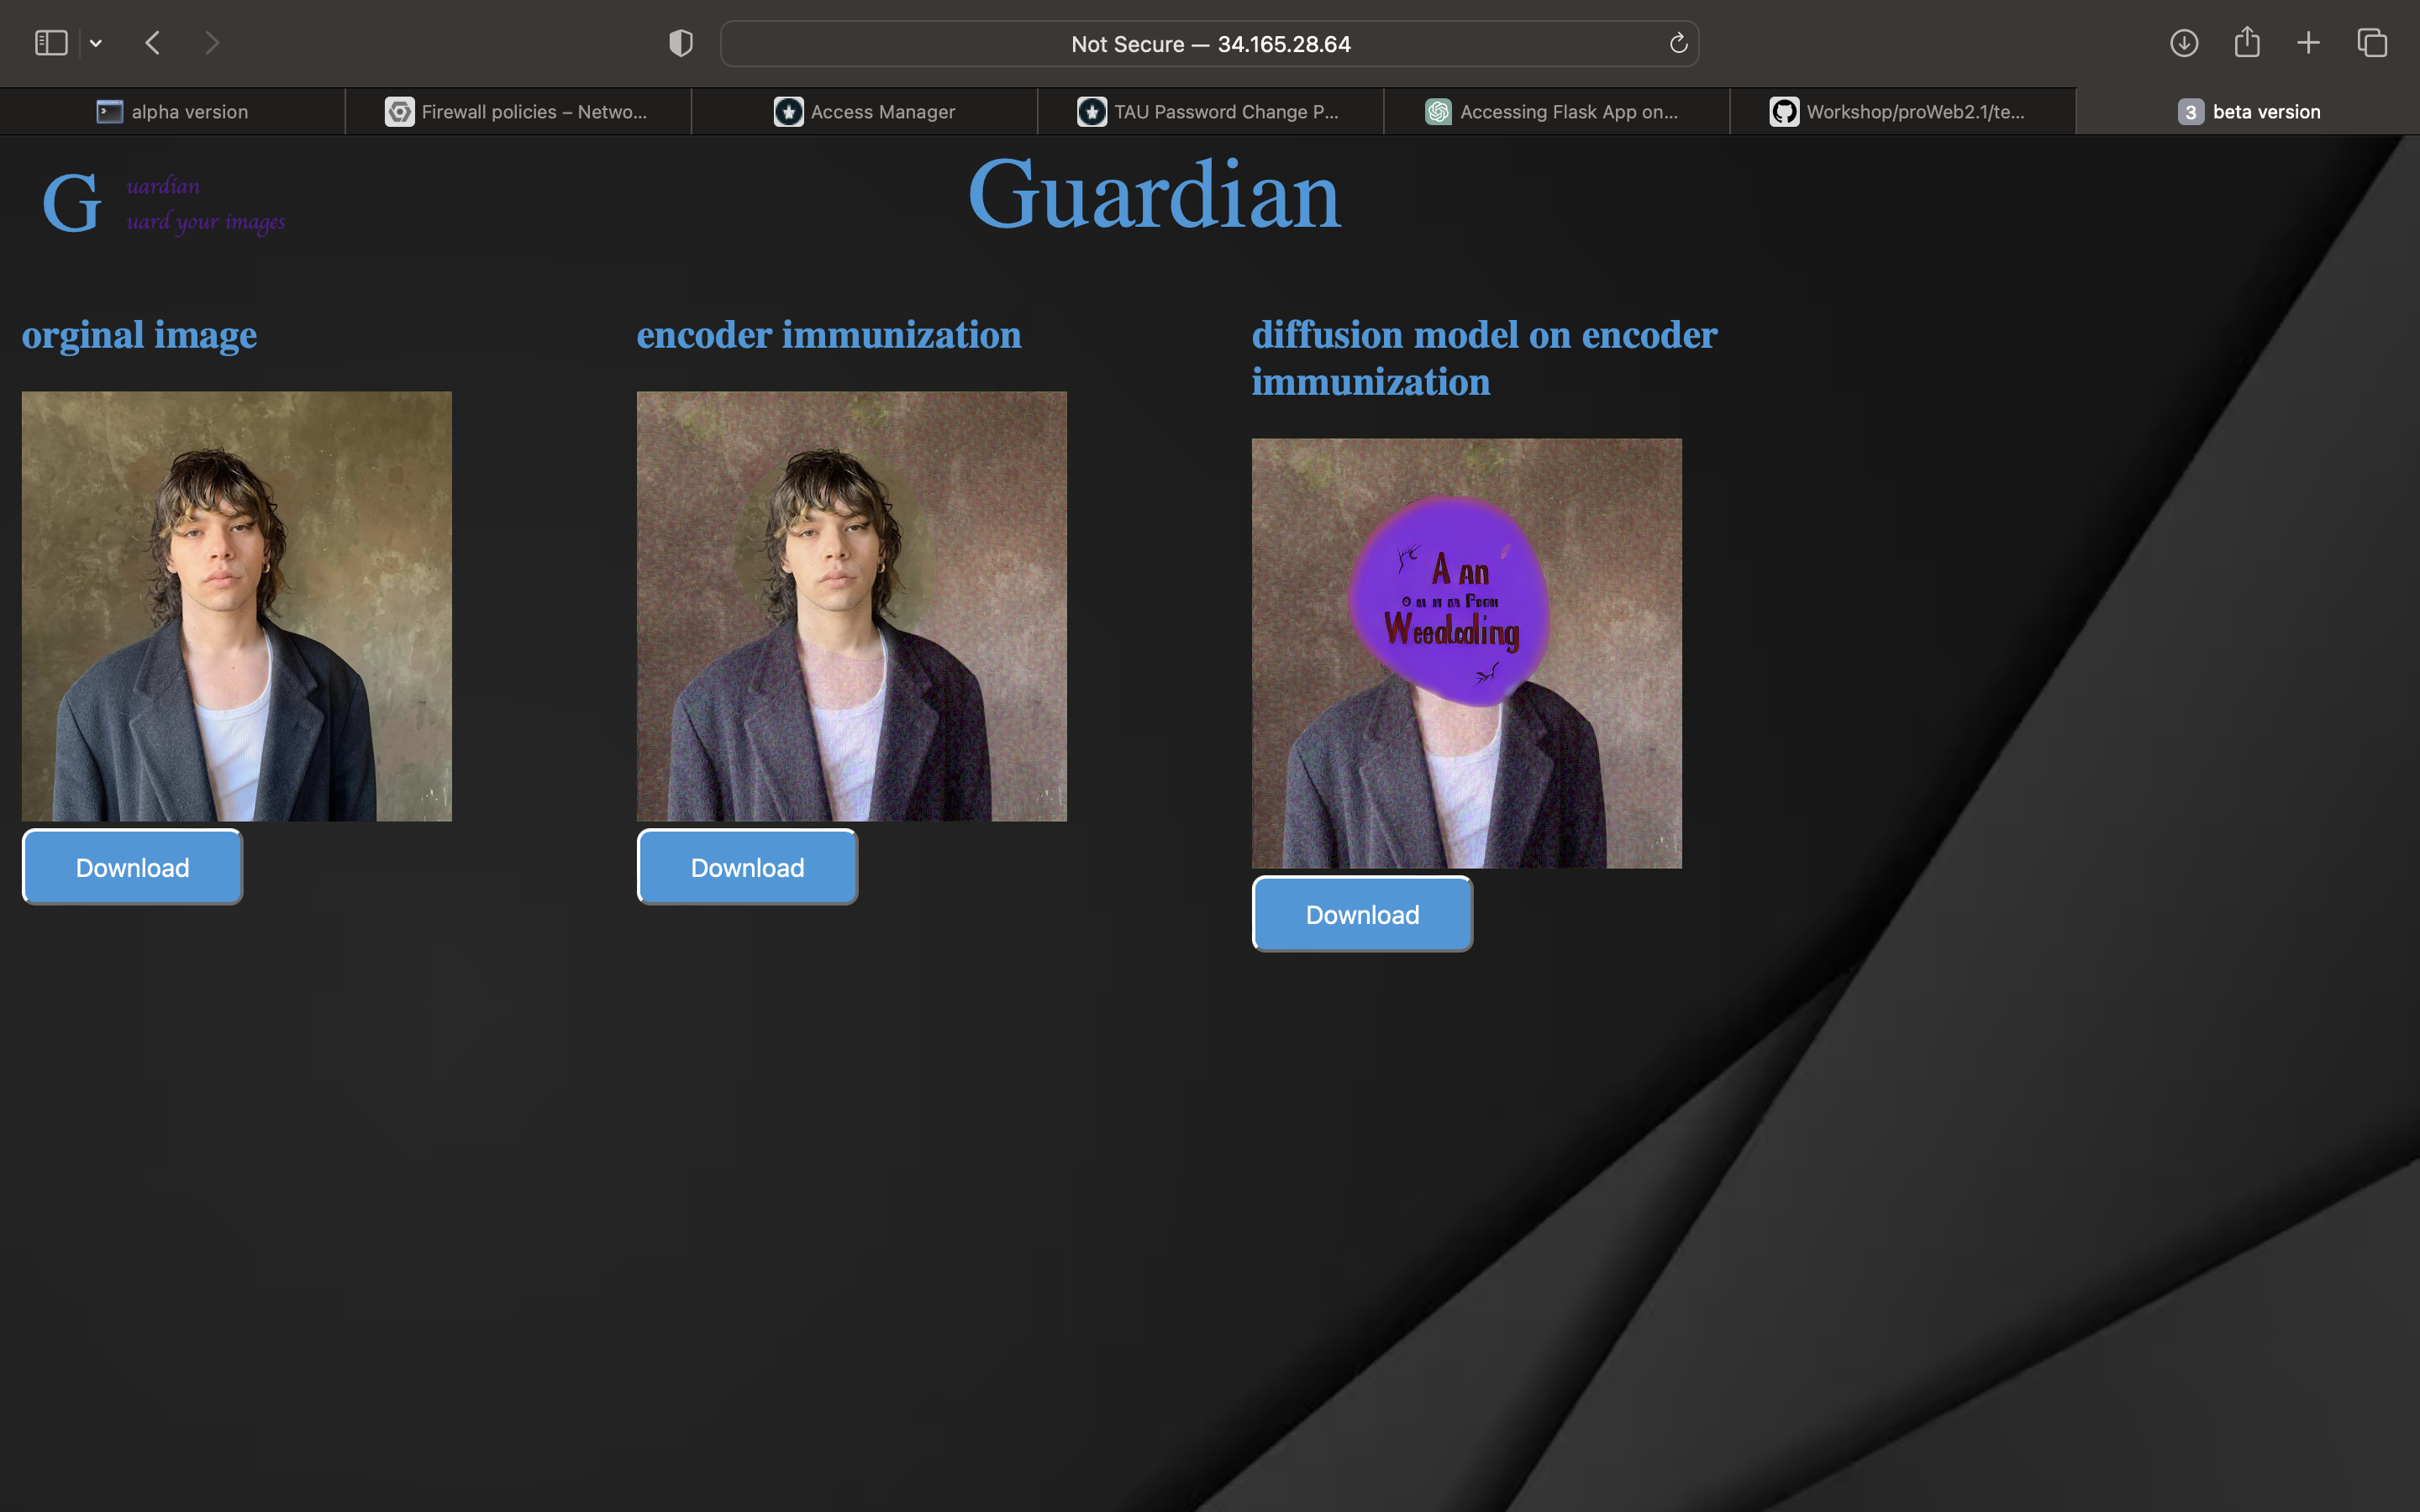
\includegraphics[width=0.4\textwidth]{5}

At the end all results is showing with the option to download the images.

\subsection{User study}

Users are the most important factor to us and we wish to reach the most postive feedback from them we want to understand how knowledgeable are they of our project subject and how much they care to guard their images, if their idea changes after the use of the web application we created, plus what they think of it how useful comfortable easy to use was it, if they would like to change anything about it, how they feel about their security and privacy, thus we need to conduct a user study. The main idea of the user study is to find out how much does making the users more involved in the process of using the AI to manipulate their images and the process of protecting said images make them feel safer and comfortable. Thus, we give users the ability to affect the process throughout the using of the web application. And asking users questions about their experience and their thoughts of the results. Our demographics of participants are young people who uses social media a lot and post a lot of images on it. we recruited people by sharing the website link and questions on social media and making people such as influencer share their experience with the people following them and suggesting people to take part in the study. We needed to make sure that our work achieved what it was set to do, so feedback from users was important to us. In our user study we focused on asking participants about their experience, what are the things they wish to change and how our work really affected their idea and feeling of confidence and security. Positive or negative feedbacks will be the stepping stone for us on how we can continue from here and change/add things to our project. 

\section{Results}

We found out that the web application can run very fast with a strong server but the diffusion attack was still taking a long time to run meaning for a proper run a very strong server is needed. In term of making the application basic we succeeded with that making it very easy to use, even people who had no Idea about the subject didn't have trouble using the application, they expressed how user friendly it was and straight to the point a lot of them appreciated the design especially the feature of description of each option in the settings page. We also noticed that styleGan was yet unable to create convincing images of images of normal users and it worked much better on celebrities' images, in addition didn't work at all for images which had no face in it or had one but was too small. Which leads us to believe that styleGan model won't be much of a trouble to everyday users, same results can be found in people reactions over styleGan they reported that it only manipulates an image of a lookalike person sometimes even a completely different person image even though no guard was used over their images. More terrifying or impressive results depends on how you look at it was recorded with the diffusion model as it succeeded in creating accurate edited images of people sometimes a very realistic images users reported their concern of it, some even did not believe this was the doing of the AI with no human hands involved. Luckly we already had the solution, the encoder attack did a very good job in protecting the images it being fast and resulted in a very impressive images where not much of a change can be seen in the original image, however when given to the AI to manipulated it, a huge change was seen as the AI couldn’t create as good of a result as the image with no encoder attack immunization, all this while still being fast and reliable. Users also expressed their satisfaction with the encoder attack saying things like "it's a life savior", we believe that the encoder attack proved itself to be a very good solution for the problem that is of today. For the diffusion attack we found it less handy and reliable as the added benefits not much better than encoder attack even sometimes resulting in a worst result, not worth the huge extra waiting time and wight put on the server, users also reported same thoughts saying the extra waiting time was not worth it and they prefer just to use the encoder attack. Thus, we believe the encoder attack won in all aspects. We must find a way to make the diffusion attack run faster or result in a better results if not we think another solution should replace it. 

At first users were more of shocked of how developed was the AI in manipulating images but using our application they did report on feeling more secure and safe after applying guard over their images and seeing the different results, in addition some even took inters in the subject of AI manipulating the images and how good the edits can be sometimes, making them search and dive deeper in this field. Users were really surprised how different it can be when immunizing the images first. When asked if they would change anything about the web application the most repeated answer was to add more AI models and immunizing methods. Even commented on the design saying they prefer if we had a light vision with more bright colors. Users also really liked the option to download all and every image they choose to create, not only the guarded image, even some used the model to edit images just for the fun of it.

\section{Discussion}

\subsection{Broader consequences}

The project can lead to a new stander of images security such that all social media platforms should use it before uploading their users' images to the internet, by that current AI models to manipulate images will be  sort of useless in editing these images. Such thing can give all internet users a sense of security in addition when we use our application that doesn't save any image or include human involvement, we created a safe and secure environment where user privacy is kept, where they can learn and touch with their own hands such technology, along the way of adding the guard layer to the images. We also did increase people awareness of such threats not only on their images but on all kind of personal data because of AI can manipulate images it surely can manipulate any kind of data, this makes users more spectacle on what they see on the internet question anything, in addition more protective over their personal data especially images, always on the look for new tools to protect all kind of their personal data. 

Such thing will help people maintain their privacy to the maximum.  
We wish to motivate future researchers to work on the problem of AI manipulating users' data and create solutions to prevent or make it harder for said AI to succeed in manipulation of such data. Even use our work and expand on it even bringing more creative ways to guard users' security and privacy.      

\subsection{limitation}

Our project is limited to a certain models and immunization methods such that anything else can cause an issue and the immunization we have might not work as intended. That being said if any new AI model which works in a different way can pass the guarding layer, we have over the images causing the users privacy to be invaded, meaning every time a new AI model that was created to manipulate images can cause users to take down all of their images and apply a new immunizing method if available by that time. Current solution today affects the images quality and protect best against one AI model so users can't really use more than one immunization method on the same image, this lead to any person who intend to use AI to manipulate image try multiple AI models until one of them result to a decent result and our work doesn't have response to it. Another limitation is our Web application is very heavy to run meaning it need a very strong server to run it this can lead to high costs to maintain it. Lastly the most obvious limitation is we only try to protect users images from AI manipulation however users still have another type of data shared all over the internet which can be targeted and manipulated by the AI models. 

\subsection{Future work and extensions}

As explained before our work is not done and this project is only the beginning, we still have a lot of ideas we are looking to add, plus the suggestions we received from users.   
 
First, we are looking to expand on the design (frontend) aspect of the web application, adding the option for users between light and dark mode, dark mode being what we have now, light mode being with white background and brighter colors, in addition we want to add more pictures, textures, texts to make the web application look more pleasant, more trustworthy, following the modern design of leading websites. We also looking to add something like the setting page, a description of everything the user sees on screen maybe even a user guide picture or even a video making our application easier to use even for younger or older people since today even they are targeted of AI manipulating their images.   

In the second aspect we are looking to expand on the backend and options to what we have right now by adding more AI based manipulation models and more methods to immunize images following the updates and new models' releases offering users first response to any new threats, plus work on what we have now try to make it better and cost less to host the web application. Try to find away to allow more than one immunization on the same image at the same time. Add more data types that we can protect especially videos. We even want to make users more part of the process by giving them more setting to be under their control since all the AI models offers a lot of settings that can result in a various result.

Another Aspect is features on our web application from small ones to large important ones, examples of such features are: 

\begin{enumerate}
  \item actuality having a loading bar with time next to it of the expected finishing time.
  \item having the option to share the images created.
  \item create a form for users to report issues.
  \item create an API for our work making it easer for other people to expand on our work.
  \item allow people to draw and paint their target image.
\end{enumerate} 

 Last thing and final goal is to share our work with social media companies where they will have their user use our work before uploading any image to their platformes.  

\section{Conclusion}

To conclude after viewing previous work and papers we created a web application (using html, css, javascript, python) in it users can  upload an image and for learning purposes use AI manipulation model to edit the image also apply immunization on these images to protect them from said AI models, at the end all of the results images can be downloaded to the user local machine .Our web application not only help users secure their images but also do so in a private safe environment where no images is saved and no human interfere in the process. We wish for more and more people to use our work to get a better idea and understand the risks if they neglected protecting their images, in addition guard their images and protect their privacy.

By the day AI are getting more advanced making the problem more dangerous, even today it is advanced enough to create realistic believable edits if images with little effort such as giving a text prompt describing the edit, we are looking to create thus the solution we offer is necessary to save users privacy, we suggest everyone to use our web application and share it to other people.

To understand users' behaviors and thoughts on the matter we conduct a user study in it we found out that after using our work they felt more secure and confident, in addition most people never heard or knew about the danger AI can posses to their privacy especially their images, they were surprised of seeing what the AI is capable of.

Currently our solution is not perfect and it still has limitations yet it still provides a good amount of protection, making it better than with no protection at all. The web application is still being developed and getting more and more advanced providing better tools for users. We shall keep track of the current situation and update our application to be able to prevent new and more advanced models from manipulating your and your love one's images. 

\section{Contributions}

Noor: frontend design, backend worked on the AI models and immunization methods, small and big features, technical report.
\newline
\newline
Ofek: frontend design, backend immunization methods, small and big features, debugging, user study, readme file.
\newline
\newline
Gali: two mid semsiter presentations, ideas for technical report and the user study.

\bibliographystyle{ACM-Reference-Format}
\bibliography{ccs-bio}

\end{document}
